
\subsection{Zoeken}\label{zoeken}

Voor \drupalpath wordt de \emph{Solr module} gebruikt, deze module vervangt de standaard \emph{Drupal Search module}. 
De \emph{Solr module} biedt naast de standaard zoek functionaliteit ook meer geavanceerde functionaliteiten zoals zoeken in bijlagen, markeren van zoekwoorden en de mogelijkheid tot het aanpassen van de \emph{Bias settings}. 

\subsubsection{Bias settings}

\emph{Bias settings} maken het mogelijk inhoud voorrang te geven in de zoekresultaten. Je kunt bijvoorbeeld het inhoudstype \emph{Nieuws} meer punten geven dan het inhoudstype \emph{Bekendmaking}. Hoe hoger het aantal toegekende punten hoe meer voorrang het krijgt. 

Ga naar \drupalpath{admin/config/search/apachesolr} en klik vervolgens op \emph{Bias} bij de betreffende website om de \emph{Bias settings} aan te passen. Let op: het is niet aangeraden om zonder voldoende kennis deze settings aan te passen.

\begin{center}
	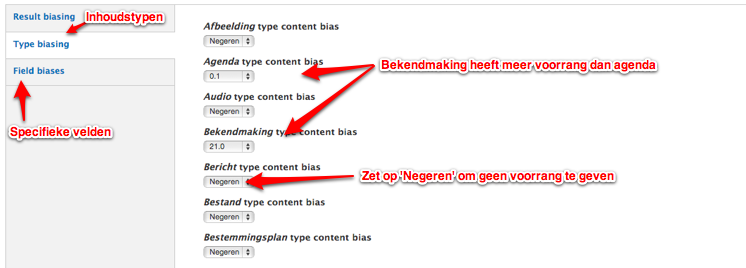
\includegraphics[width=\textwidth]{img/bias.png}
\end{center}

Klik na het bewerken op de knop \emph{Instellingen opslaan} om de \emph{Bias settings} op te slaan. 

\subsubsection{Content uitsluiten van zoekmachine}

Het is mogelijk om specifieke nodes uit te sluiten van indexatie in de interne zoekmachine. Klik onderaan het bewerkformulier op het tabblad \emph{Uitsluiten uit zoekresultaten} en vink de checkbox aan, zie onderataand afbeelding.

\begin{center}
	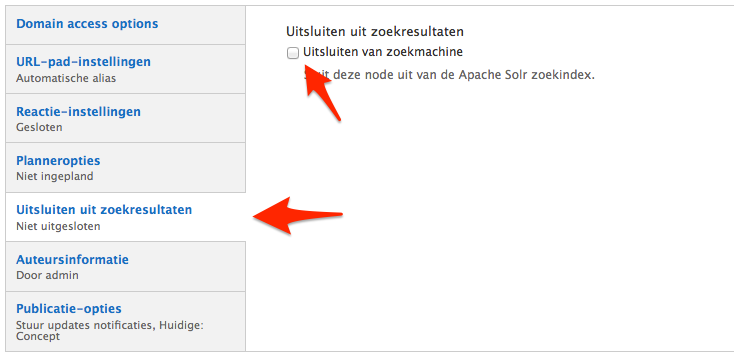
\includegraphics[width=\textwidth]{img/solr-exclude.png}
\end{center}

\subsubsection{Synoniemen beheren}

Solr biedt ondersteuning voor synoniemen. Hiermee kan worden ingesteld dat een zoekopdracht naar "i-pad" ook inhoud met de tekst \emph{ipad} wordt opgenomen in de resultaten.

De synoniemen zijn te beheren via Drupal. Ga hiervoor naar \\ \drupalpath{admin/config/search/apachesolr/synonyms}. Op deze pagina is een lijst te vinden met de huidige synoniemen. Deze kunnen hier worden aangepast of uit de lijst worden gehaald. Onder de lijst is een formulier zichtbaar waarmee nieuwe synoniemen toegevoegd kunnen worden. Het trefwoord is het originele woord (bijv. \emph{ipad}) en de synoniemen worden ingevoerd als een komma gescheiden lijst (bijv. "i-pad, i pad").

Nieuwe synoniemen treden niet direct in werking. De lijst wordt iedere nacht doorgezet naar de Solr server. In dit proces wordt tevens de ingestelde lijst samengevoegd met de basislijst (generieke lijst voor alle gemeentes).
